\documentclass[14pt,a4paper]{article}

\usepackage[utf8]{inputenc}
\usepackage[
backend=biber,
style=ieee,
natbib=true,
sorting=nyt,
url=false,
isbn=false,
doi=true
]{biblatex}
\addbibresource{bibliography.bib}
\usepackage[english,russian]{babel}
\usepackage[T2A]{fontenc}
\usepackage{graphicx}
\usepackage{amssymb}
\usepackage{amsthm}
\usepackage{amsmath}
\usepackage{bm}
\graphicspath{{media}}
\usepackage{float}
\usepackage{caption} % пакет для работы с названиями плавающих элементов
\usepackage{}
%\setlength{\parindent}{1.25cm}
\usepackage{indentfirst}
\usepackage[a4paper,
%showframe, % отображение границ области листа
top		=	2.00cm,
bottom	=	2.00cm,
left	=	3.00cm,
right	=	1.50cm,
nohead,
foot	=	0.75cm
]{geometry} % пакет формата листа

\setlength{\parindent}{1.25cm} % задаём размер красной строки
\usepackage{setspace} % пакет для работы с интервалами
\onehalfspacing % полуторный интервал

\begin{document}
    
    \section*{Аннотация}

        В данной работе рассматривалась оригинальная конструкция гидродинамического диода в котором основным исследуемым параметром был выбран угол наклона отводящего канала. Численно исследован стационарный режим течения несжимаемой линейно-вязкой жидкости. Получена зависимость диодности устройства от угла наклона отводящего канала. Рассмотрен вопрос сеточной сходимости решения. Выбраны оптимальные параметры расчетной сетки.

    \section*{Введение.}

        Характерной особенностью гидродинамических диодов, так же известных как клапаны Тесла \cite{JIN20188888}, является то, что при заданном расходе флюида необходимо прикладывать разный перепад давления в зависимости от направления потока. Данные устройства нашли широкое применение в науке и технике поскольку сочетают в себе простоту конструкции за счет отсутствия механических подвижных частей и эффективность. Клапаны такого типа обладают такими преимуществами как масштабируемость [], долговечность [] и простота изготовления из различных материалов [].

        Обзор...

        %Это обратный клапан в котором отсутствуют механические подвижны части. Клапаны такого типа обладают такими преимуществами как масштабируемость, долговечность и простота изготовления из различных материалов. Гидравлические диоды препятствуют току жидкости при обратном подключении и создают заметно меньше сопротивления при прямом подключении.

        %В данной работе будет рассмотрен клапан Тесла, который является гидравлическим диодом. Это обратный клапан в котором отсутствуют механические подвижны части. Клапаны такого типа обладают такими преимуществами как масштабируемость, долговечность и простота изготовления из различных материалов. Гидравлические диоды препятствуют току жидкости при обратном подключении и создают заметно меньше сопротивления при прямом подключении.

        %По ходу работы мы рассмотрим теорию и математическую модель решателя SimpleFoam пакета OpenFoam, будет проведено параметрическое исследование. Цель состоит в том, чтобы максимизировать диодность клапана Тесла путем изменения параметров.

        %Прежде чем приступить к параметрическому исследованию мы провели исследование сеточной сходимости, чтобы определить оптимальное разрешение расчетной сетки для дальнейшей работы. Ошибки дискретизации уменьшаются при увеличении степени детализации сетки. И можно ожидать, что при достижении некоторой степени детализации сетки дальнейшее увеличение уровня детализации не приведет к заметному улучшению численного решения. Наша цель на этом этапе -- определить разрешение, при котором дальнейшее увеличение детализации сетки не будет приводить к значительным улучшениям результатов расчета. Оба эти этапа объедены общей идей, создать модель для исследование с минимальным количеством независимых параметров.
        
    
    \section*{Геометрия расчетной области и расчетная сетка}

        В настоящее время существует множество различных вариаций клапана Теслы, заметно отличающихся от оригинальной версии, представленной в патенте US1329559A самим Николо Тесло. В нашем исследовании используется следующая вариация клапана Теслы:

        \begin{figure}[h!]
            \centering
            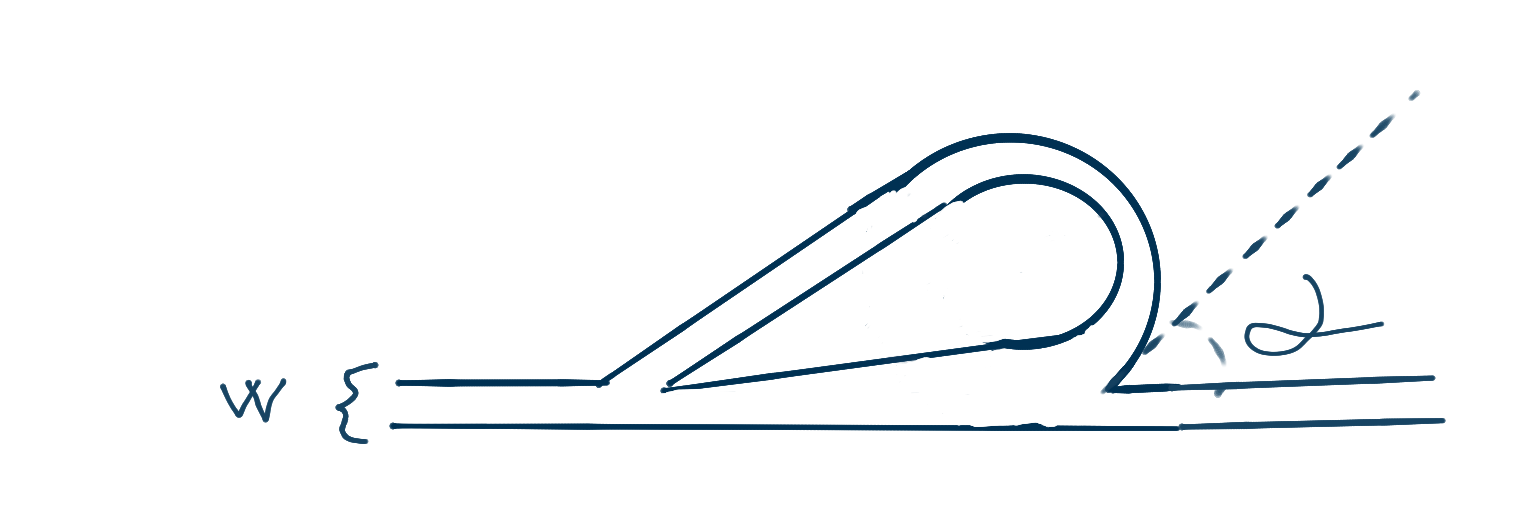
\includegraphics[width=100mm,scale=0.5]{teslaValve}
            \caption{Клапан Тесла.}
            \label{fig:TeslaValve}
        \end{figure}
        Это прямой канал с U-образным отводным каналом. Задача отводного канала, разделить ток жидкости идущей по основному каналу, и перенаправить отведенную часть против основного потока. Таким образом, клапан Тесла, при обратном подключении и работает, замедляя ток жидкости. Заметным отличием от оригинальной версии клапана Теслы является явно выделенный основной канал, к которому добавлены отводящие каналы.          
        
        На основе выбранного шаблона был написан скрипт на языке Python, для построения параметрической геометрии и расчетной сетки с минимальным количеством независимых параметров. Основной параметр для параметрического исследования -- это угол $ \alpha  $, а для исследования сеточной сходимости -- это максимальный характерный размер одной ячейки сетки, в микрометрах.
       
        
        \begin{figure}[h!]
            \centering
            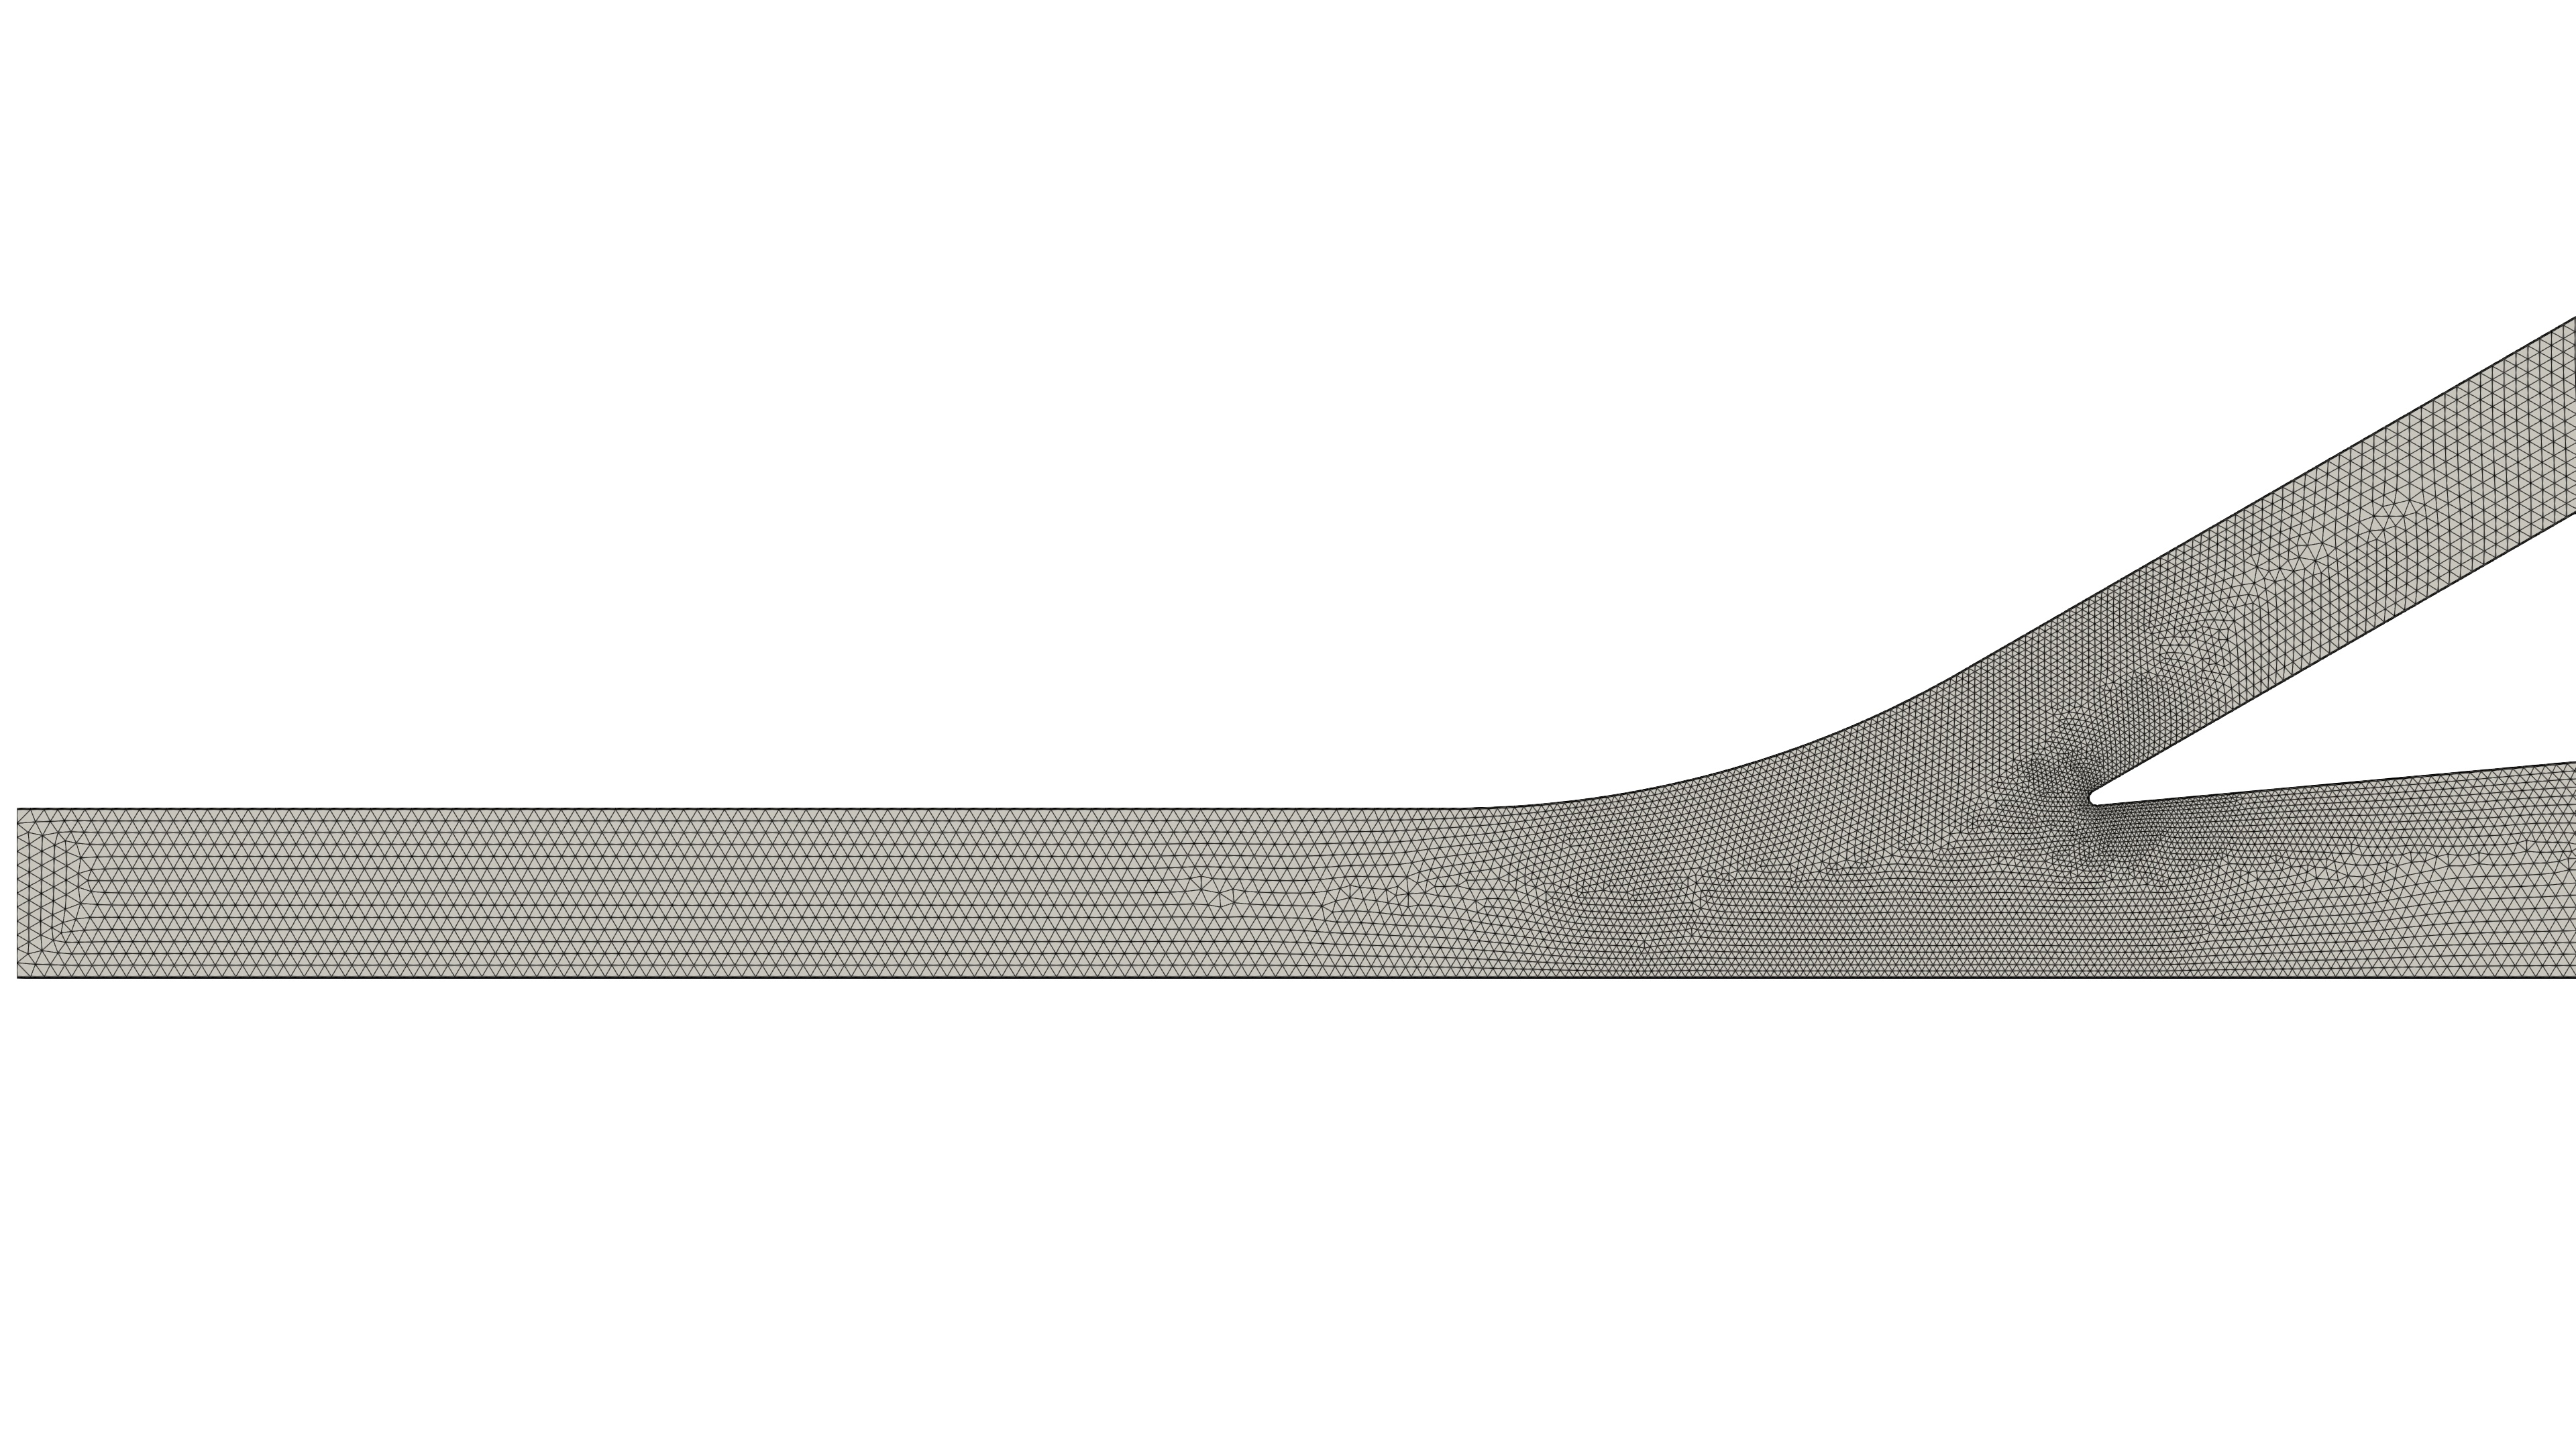
\includegraphics[width = 1\linewidth]{teslaMesh1}
            \caption{Расчетная сетка.}
            \label{fig:teslaMesh}
        \end{figure}
        
        На (рис.~\ref{fig:teslaMesh}) угол $\alpha$ равен 30 градусам, ширина канала была выбрана равной 500 мкм или 0.0005 м. Также, можно видеть, что сетка не однородная. В нашей задаче основной интерес сосредоточен в областях, где поток разделяется и перемешивается. В них могут происходить отрывы или скачки, для разрешения градиентов давления и более точного определения профиля скорости разрешение сетки в этих областях выше.
        
        \begin{figure}[H]
            \centering
            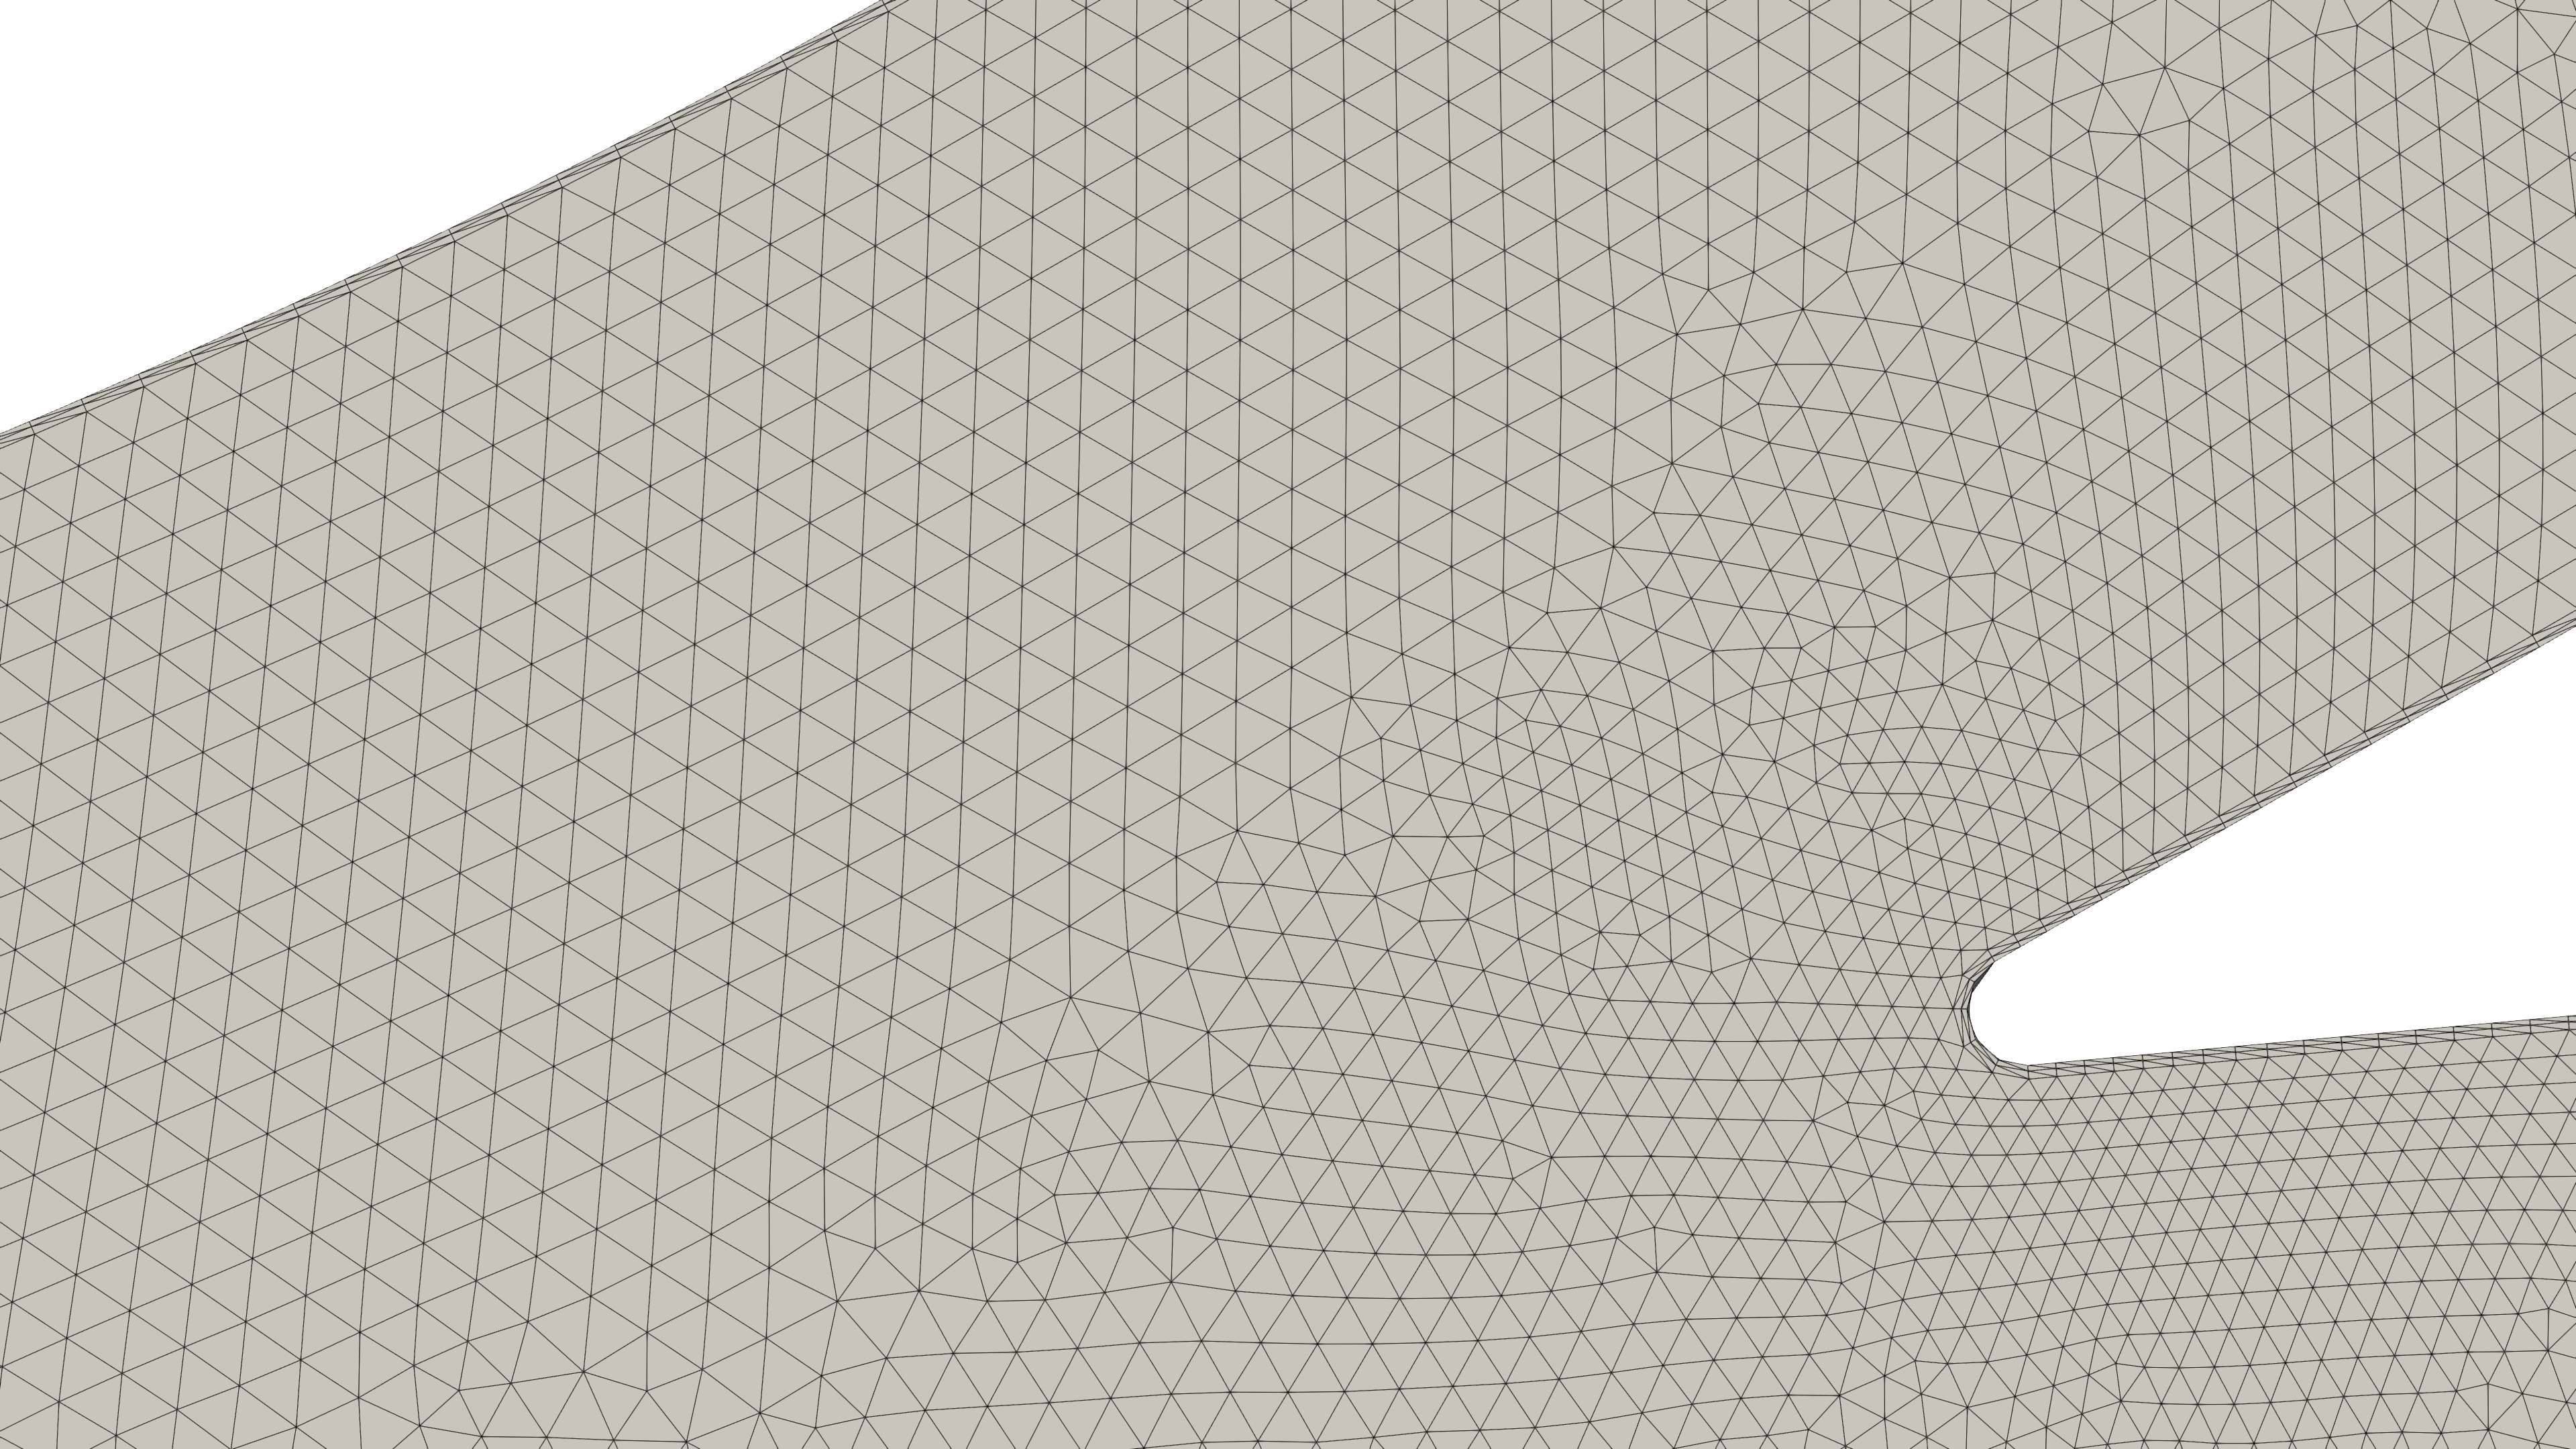
\includegraphics[width = 1\linewidth]{teslaMesh2}
            \caption{Расчетная сетка в приближении.}
            \label{fig:teslaMesh2}
        \end{figure}   
             
        Для разрешения градиента скорости вблизи стенок был добавлен сеточный подслой (рис.~\ref{fig:teslaMesh2}).
        
    \section*{Режим течения и расчет.}        
        
        Чтобы определить какого рода перед нами течение, можно рассчитать число Рейнольдса, Re. Исходя из полученного значения, можно будет сделать выводы о характере потока, турбулентное или ламинарное.
        Так как канал нашей конфигурации клапана Теслы имеет квадратное сечение, то формула для определения числа Рейнольдса имеет вид:
        
        \begin{equation}\label{eqn:Re}
            Re = \frac{u D_{H}}{\nu},
        \end{equation}            
        где  u - скорость в канале, м/с, $ D_{H} = \frac{4A}{P} $ - гидравлический диаметр, м, $\nu$ - кинематическая вязкость, м$^{2}/$с. 
        где A - площадь поперечного сечения канала, м$^{2}$, P - смоченный периметр. 
        
        Для нашей конфигурации была выбрана скорость, задаваемая на входе, равной 3 м/с, а число соответственно равно Рейнольдса - 1500.
        
        OpenFoam - это открытый программный комплекс для решения задач механики сплошной среды. SimpleFoam - это стационарный решатель для несжимаемого турбулентного потока, использующий алгоритм SIMPLE. Математическая модель, реализованная в решателе SimpleFoam, имеет вид:
        
        \begin{equation}\label{eqn:simpleFoam}
            \bm{\nabla} \cdot \bm{u} = 0
        \end{equation} 
        
        \begin{equation}\label{eqn:simpleFoam2}
            \bm{\nabla} \cdot \bm{u} \otimes \bm{u} = -\bm{\nabla} p + \bm{\nabla} \cdot \bm{\tau}
        \end{equation} 
        
        Где $\bm{u}$ - скорость, м/с, p - кинематическое давление, м$^{2}/$с$^{2}$, $\bm{\tau}$ - тензор напряжения. 
        Каждый цикл итерации влечет за собой сначала расчет промежуточного поля скорости, которое удовлетворяет линеаризованным уравнениям импульса для предполагаемого распределения давления: затем применяется принцип сохранения массы для настройки скоростей и давлений, так что все уравнения находятся в равновесии.
        
%       По графику невязок (рис.~\ref{fig:DRLam}) видно, что, при расчете без использования модели турбулентности, решение является неустойчивым. 
%        
%        \begin{figure}[H]
%            \centering
%            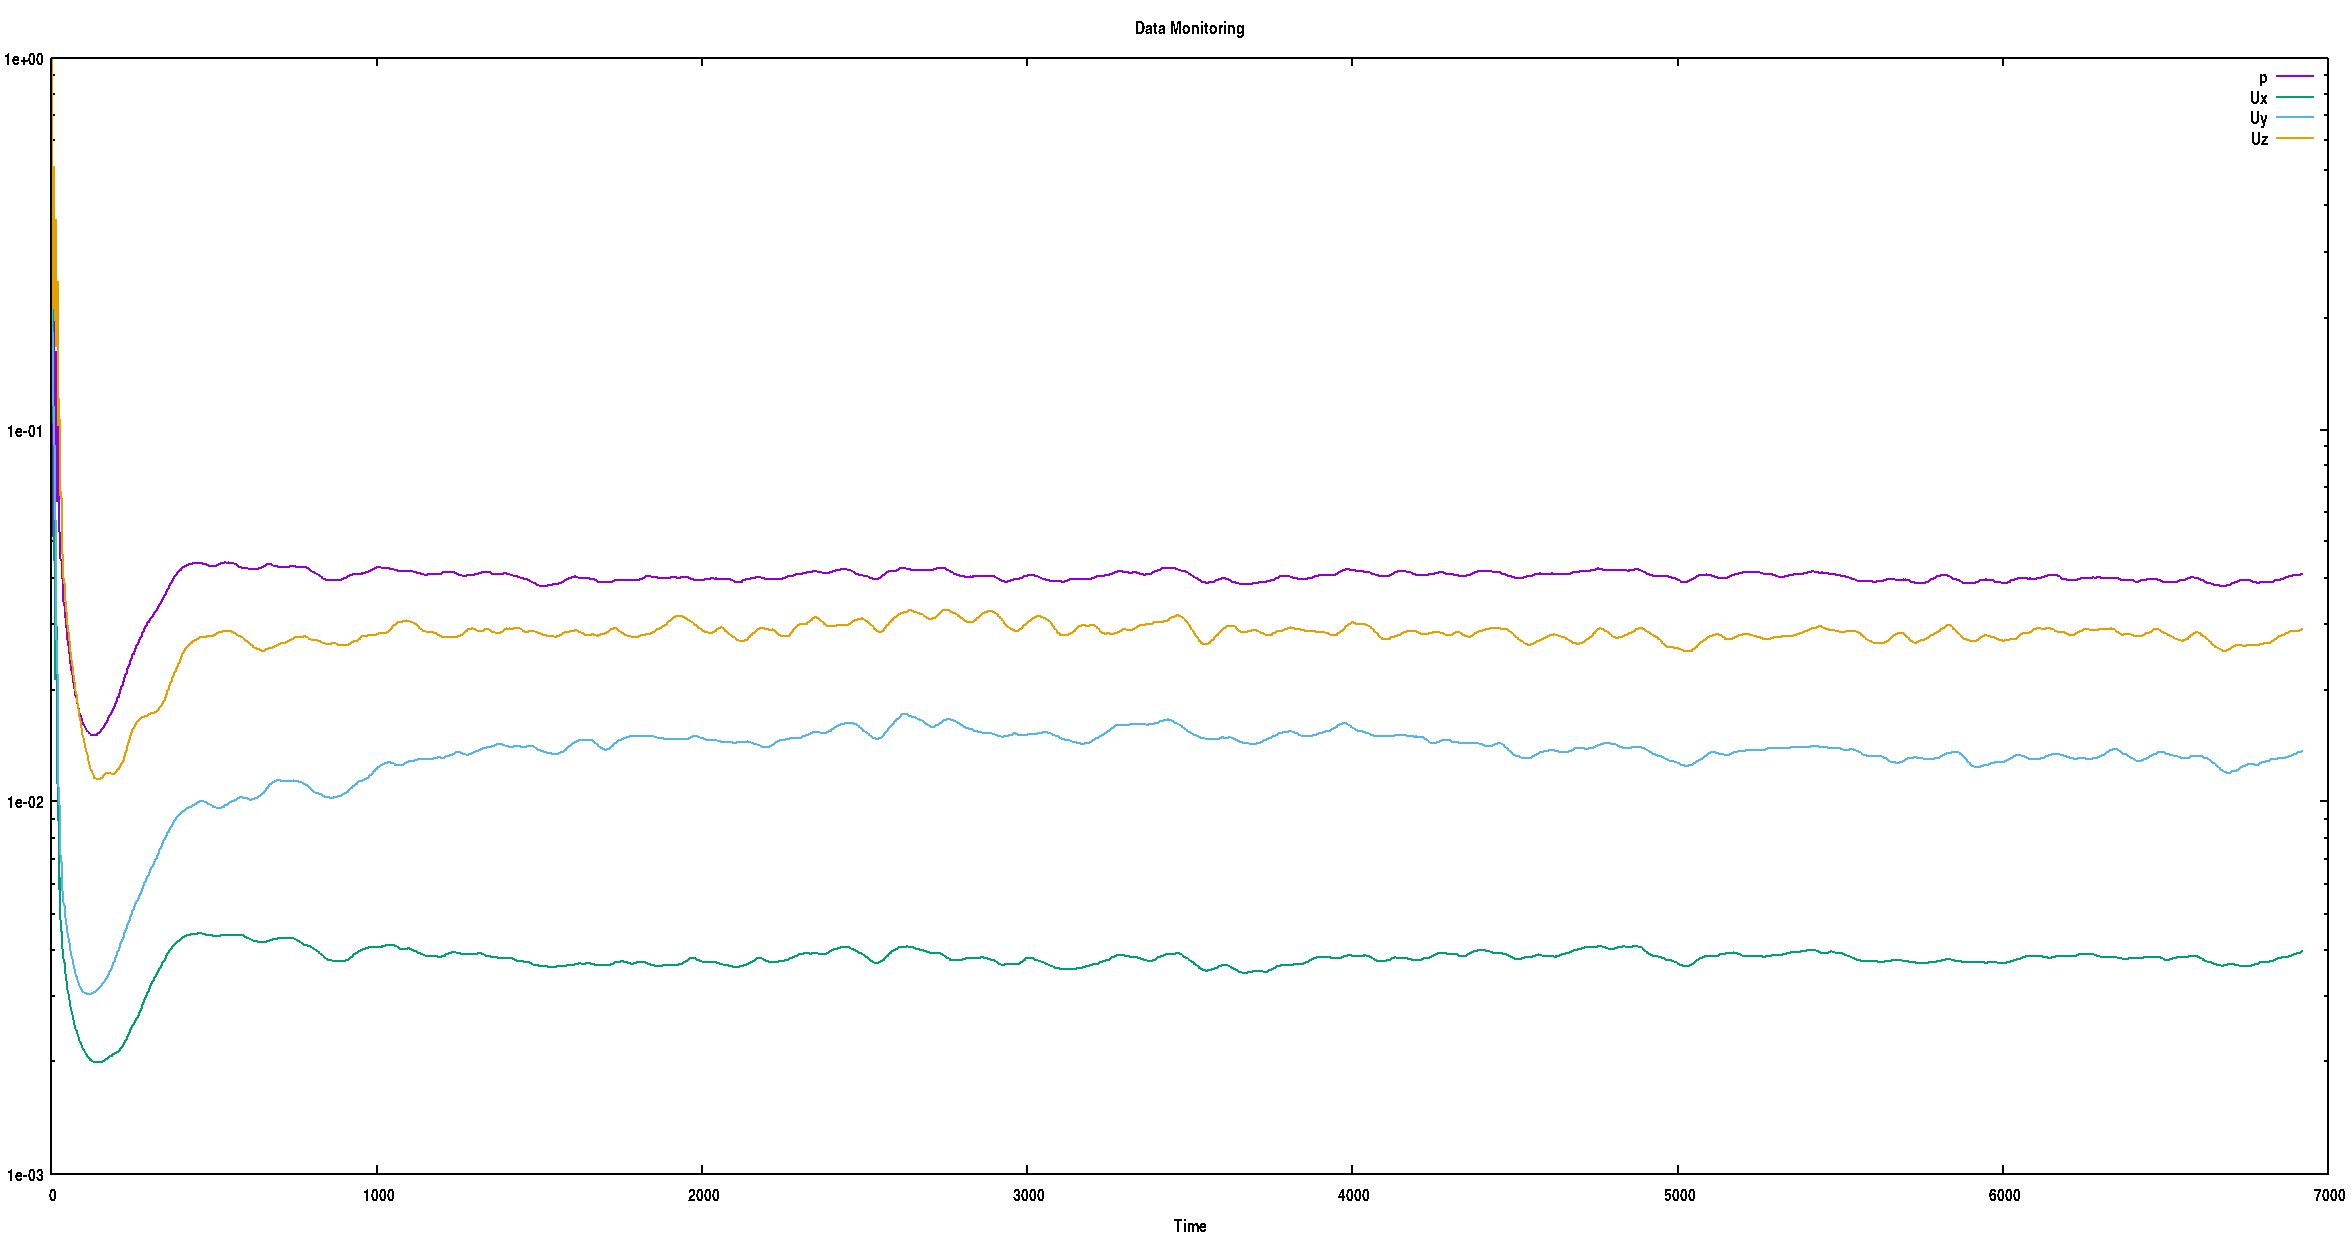
\includegraphics[width = 1\linewidth]{dataMonitoringLaminar}
%            \caption{Сходимость с ламинарной моделью.}
%            \label{fig:DRLam}
%        \end{figure}
%        
%        
%        Исходя из этого было принято решение о подключении турбулентной модели k-epsilon. Выбранным типом моделирования турбулентности был параметр RAS. Модель k-epsilon объединяет уравнения турбулентной кинетической энергии (\ref{eqn:k}), k, и уравнение скорости рассеивания турбулентной кинетической энергии (\ref{eqn:e}), $\epsilon$.
        
        Выбранным типом моделирования турбулентности был параметр RAS. Модель k-epsilon объединяет уравнения турбулентной кинетической энергии (\ref{eqn:k}), k, и уравнение скорости рассеивания турбулентной кинетической энергии (\ref{eqn:e}), $\epsilon$.
        
        \begin{equation}\label{eqn:k}
            \frac{D}{D_{t}}(\rho k) = \nabla \cdot (\rho D_{k}\nabla k) + P - \rho\epsilon
        \end{equation} 
        
        \begin{equation}\label{eqn:e}
            \frac{D}{D_{t}}(\rho\epsilon) = \nabla \cdot (\rho D_{\epsilon}\nabla\epsilon) + \frac{C_{1}\epsilon}{k}(P + C_{3}\frac{2}{3}k\nabla \cdot \bm{u}) - C_{2}\rho\frac{\epsilon^2}{k}
        \end{equation} 
       Где k --- турбулентная кинетическая энергия, м$^2$/с$^2$, $D_{k}$ - Эффективная диффузионная способность для k, P - скорость производства турбулентной кинетической энергии, м$^2$/с$^-3$, $\epsilon$ - скорость рассеивания турбулентной кинетической энергии, м$^2$/с$^-3$, $D_{\epsilon}$ - Эффективная диффузионная способность для $\epsilon$.
               
        Далее решается уравнение для турбулентной вязкости:
        
        \begin{equation}\label{eqn:mu}
           \nu_{t} = C_{\mu}\frac{k^2}{\epsilon}
        \end{equation} 
        Где $C_{\mu}$ - модельный коэффициент турбулентной вязкости, $\mu_{t}$ - турбулентная вязкость, м$^2$/с$^-1$.
        
%        В результате, мы видим, что график невязок, при подключенной модели турбулентности k-epsilon, показывает нам устойчивое решение (рис.~\ref{fig:DRRAS}).  
%        
%        \begin{figure}[H]
%            \centering
%            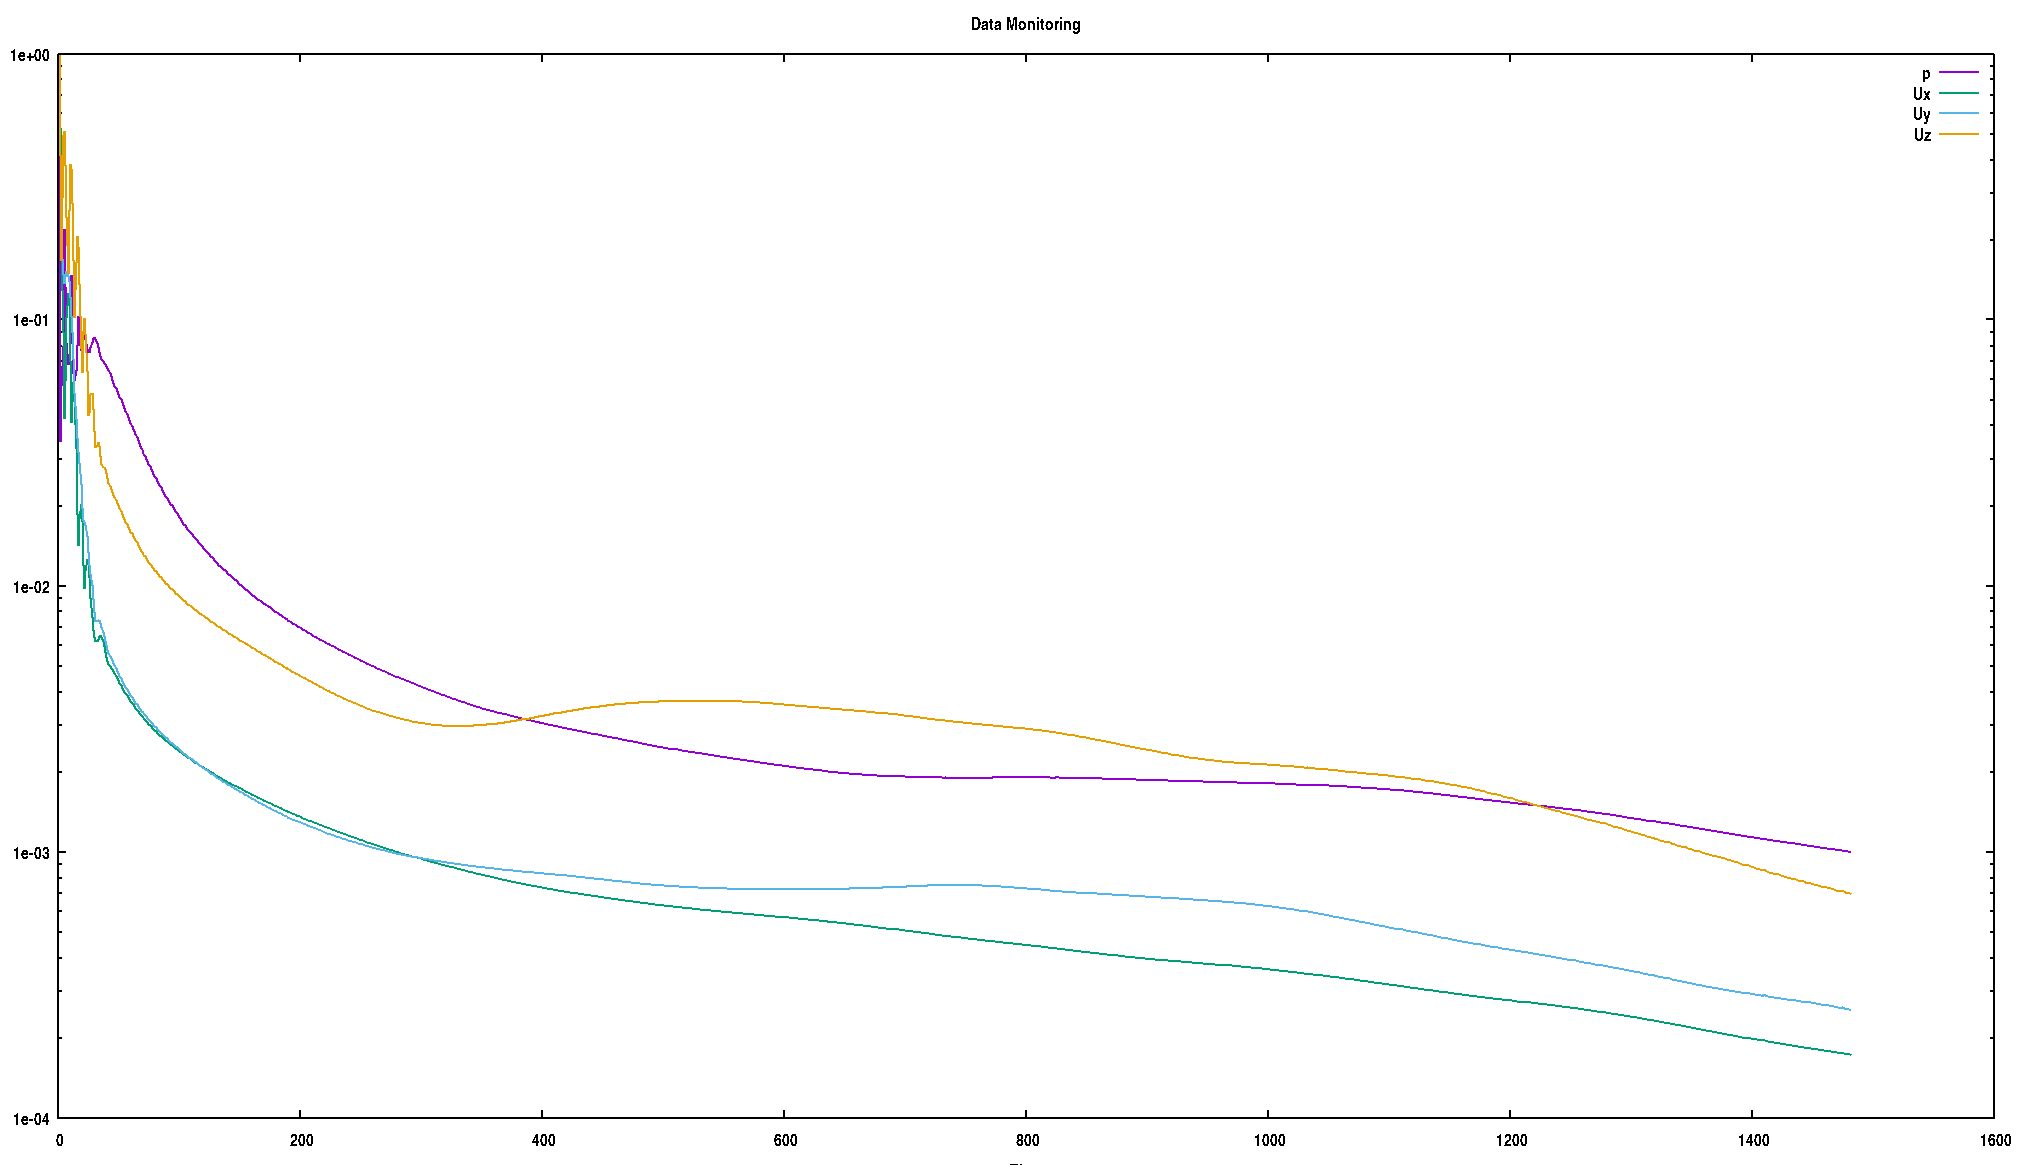
\includegraphics[width = 1\linewidth]{dataMonitoringRAS}
%            \caption{Сходимость с моделью турбулентности.}
%            \label{fig:DRRAS}
%        \end{figure}
        
        Граничные условия для решения уравнений турбулентности заданы через интенсивность для k (\ref{eqn:kI}) и через длину перемешивания для $\epsilon$ (\ref{eqn:el}). Граничные условия для скорости заданы через объемный расход, для давления через абсолютное давление (\ref{eqn:P0}).
        
        \begin{equation}\label{eqn:kI}
            k_{p} = 1.5 (I |U|)^2
        \end{equation}
        Где $k_{p}$ - кинетическая энергия на границе, м$^2$/с$^2$, I - интенсивность турбулентности.
        
        \begin{equation}\label{eqn:el}
            \epsilon_{p} = \frac{C_{\mu}^{0.75} k^{1.5}}{L}           
        \end{equation}
        Где $\epsilon_{p}$ - диссипация кинетической энергии на границе, м$^2$/с$^-3$, L - шкала длины.
        
        \begin{equation}\label{eqn:P0}
            p_{p} = p_{0} + \frac{1}{2}\ \left|u_{0}\right|^2 - \frac{1}{2}\ \left|u\right|^2
        \end{equation}
        Где $p_{p}$ - давление на границе, м$^{2}/$с$^{2}$, $p_{0}$ - внешнее статическое давление, м$^{2}/$с$^{2}$, $u$ - скорость, м/с, $u_{0}$ - внешняя скорость, м/с.\\
        
        Оценить с эффективность клапана Теслы, после получения результатов расчета, мы можем, посчитав его диодность, Di (\ref{eqn:Di}). Если Di > 1, то рассматриваемый клапан можно считать рабочим. Для этого мы проводили расчет нашей конфигурации клапана Тесла с одинаковыми параметрами дважды, но при разных подключениях: при обратном, когда перепад давления наибольший, и, при прямом, когда перепад давления наименьший. Полученные данные фиксировались.         
        
        \begin{equation}\label{eqn:Di}
            Di = (\frac{\bigtriangleup p_{r}}{\bigtriangleup p_{f}})_Q
        \end{equation}
        Где $\bigtriangleup p_{r}$ - перепад давления при обратном подключении, $\bigtriangleup p_{f}$ - перепад давления при прямом подключении для скорости потока Q.
        
        \section*{Результаты.}
        
        При выборе минимального разрешения сетки, мы остановились на таком разрешении, которое позволяло бы на входе поместиться 5 ребрам ячеек расчетной сетки (рис.~\ref{fig:minMesh}). Такое решение было принято в пользу лучшей сходимости задачи.
        
        \begin{figure}[H]
            \centering
            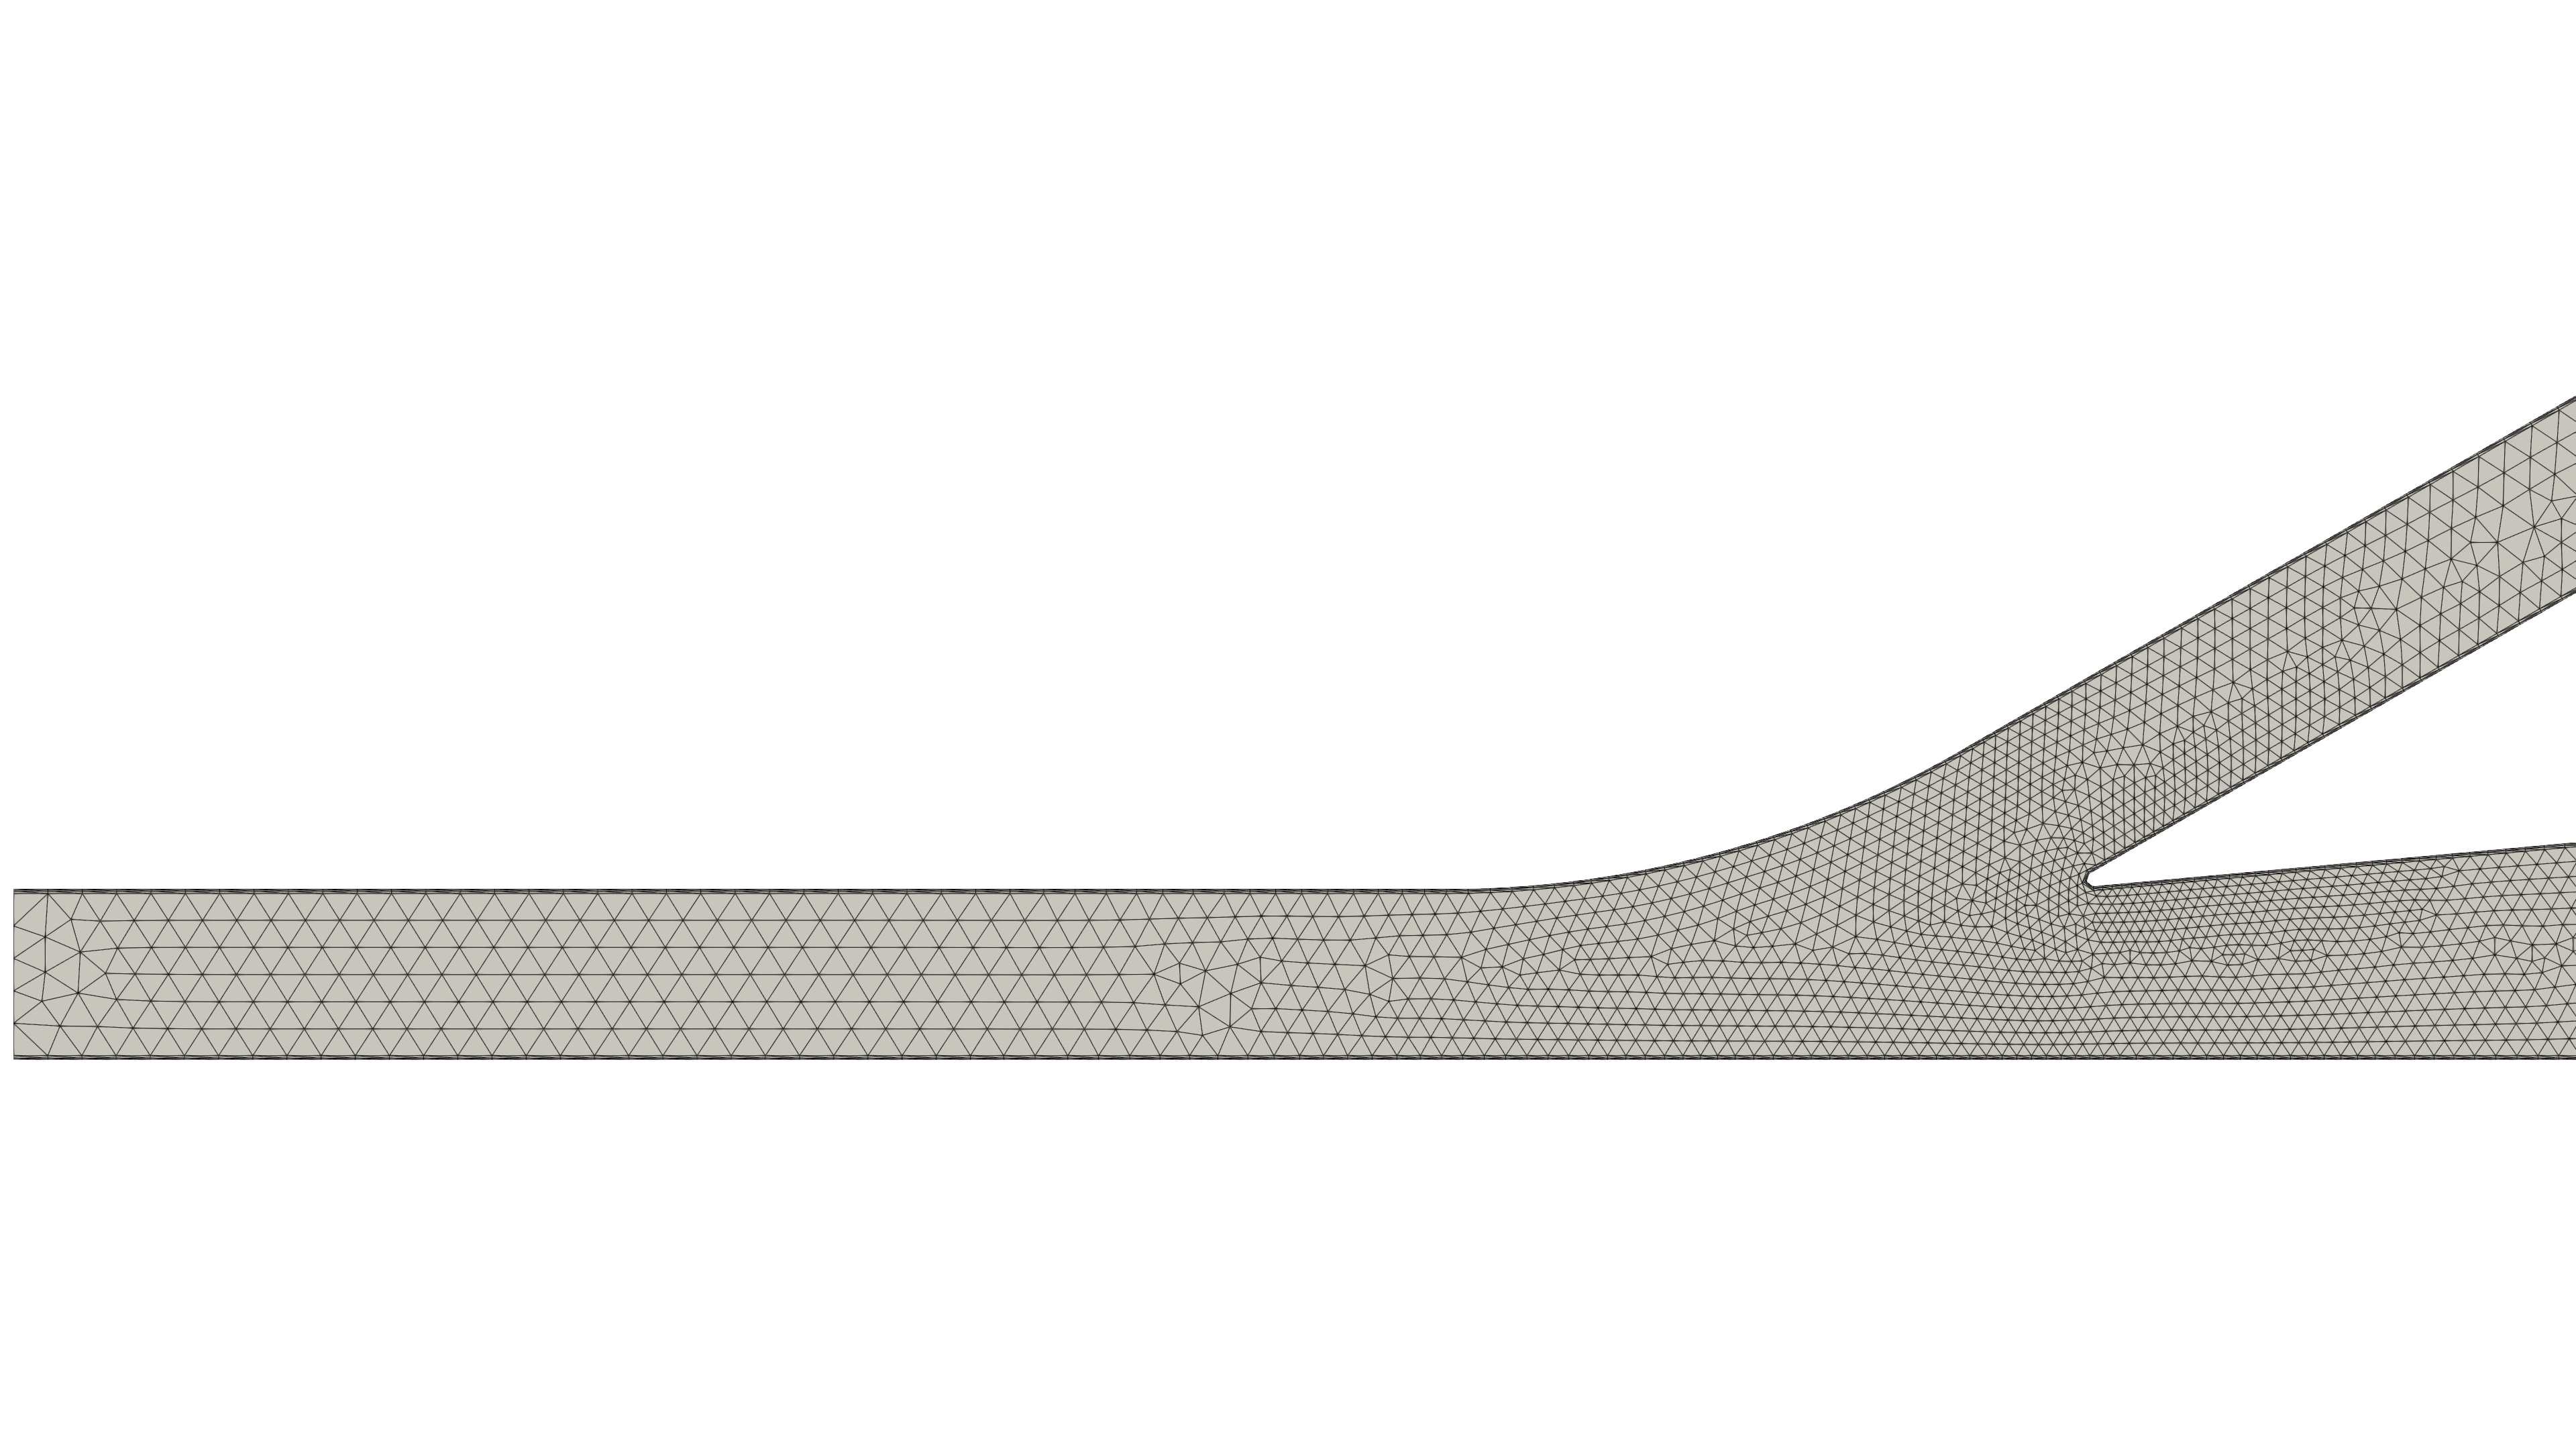
\includegraphics[width = 1\linewidth]{minMesh}
            \caption{Минимальное разрешение сетки.}
            \label{fig:minMesh}
        \end{figure}
        
        Рассмотрим полученные в ходе расчетов поля давления (рис.~\ref{fig:PFieldsReverse}) и скорости (рис.~\ref{fig:UFieldsReverse}) при обратном подключении. На изображении поля давления видно, как по мере удаления от входа, давление в клапане снижается и имеет вид приближенный к линейному. Видно, как в местах где поток разделяется и смешивается, происходят скачки давления. Изображение поля скорости, демонстрирует нам значительное падание скорости между участками клапана, где происходит разделение и смешивание потоков жидкости.
        
        \begin{figure}[H]
            \centering
            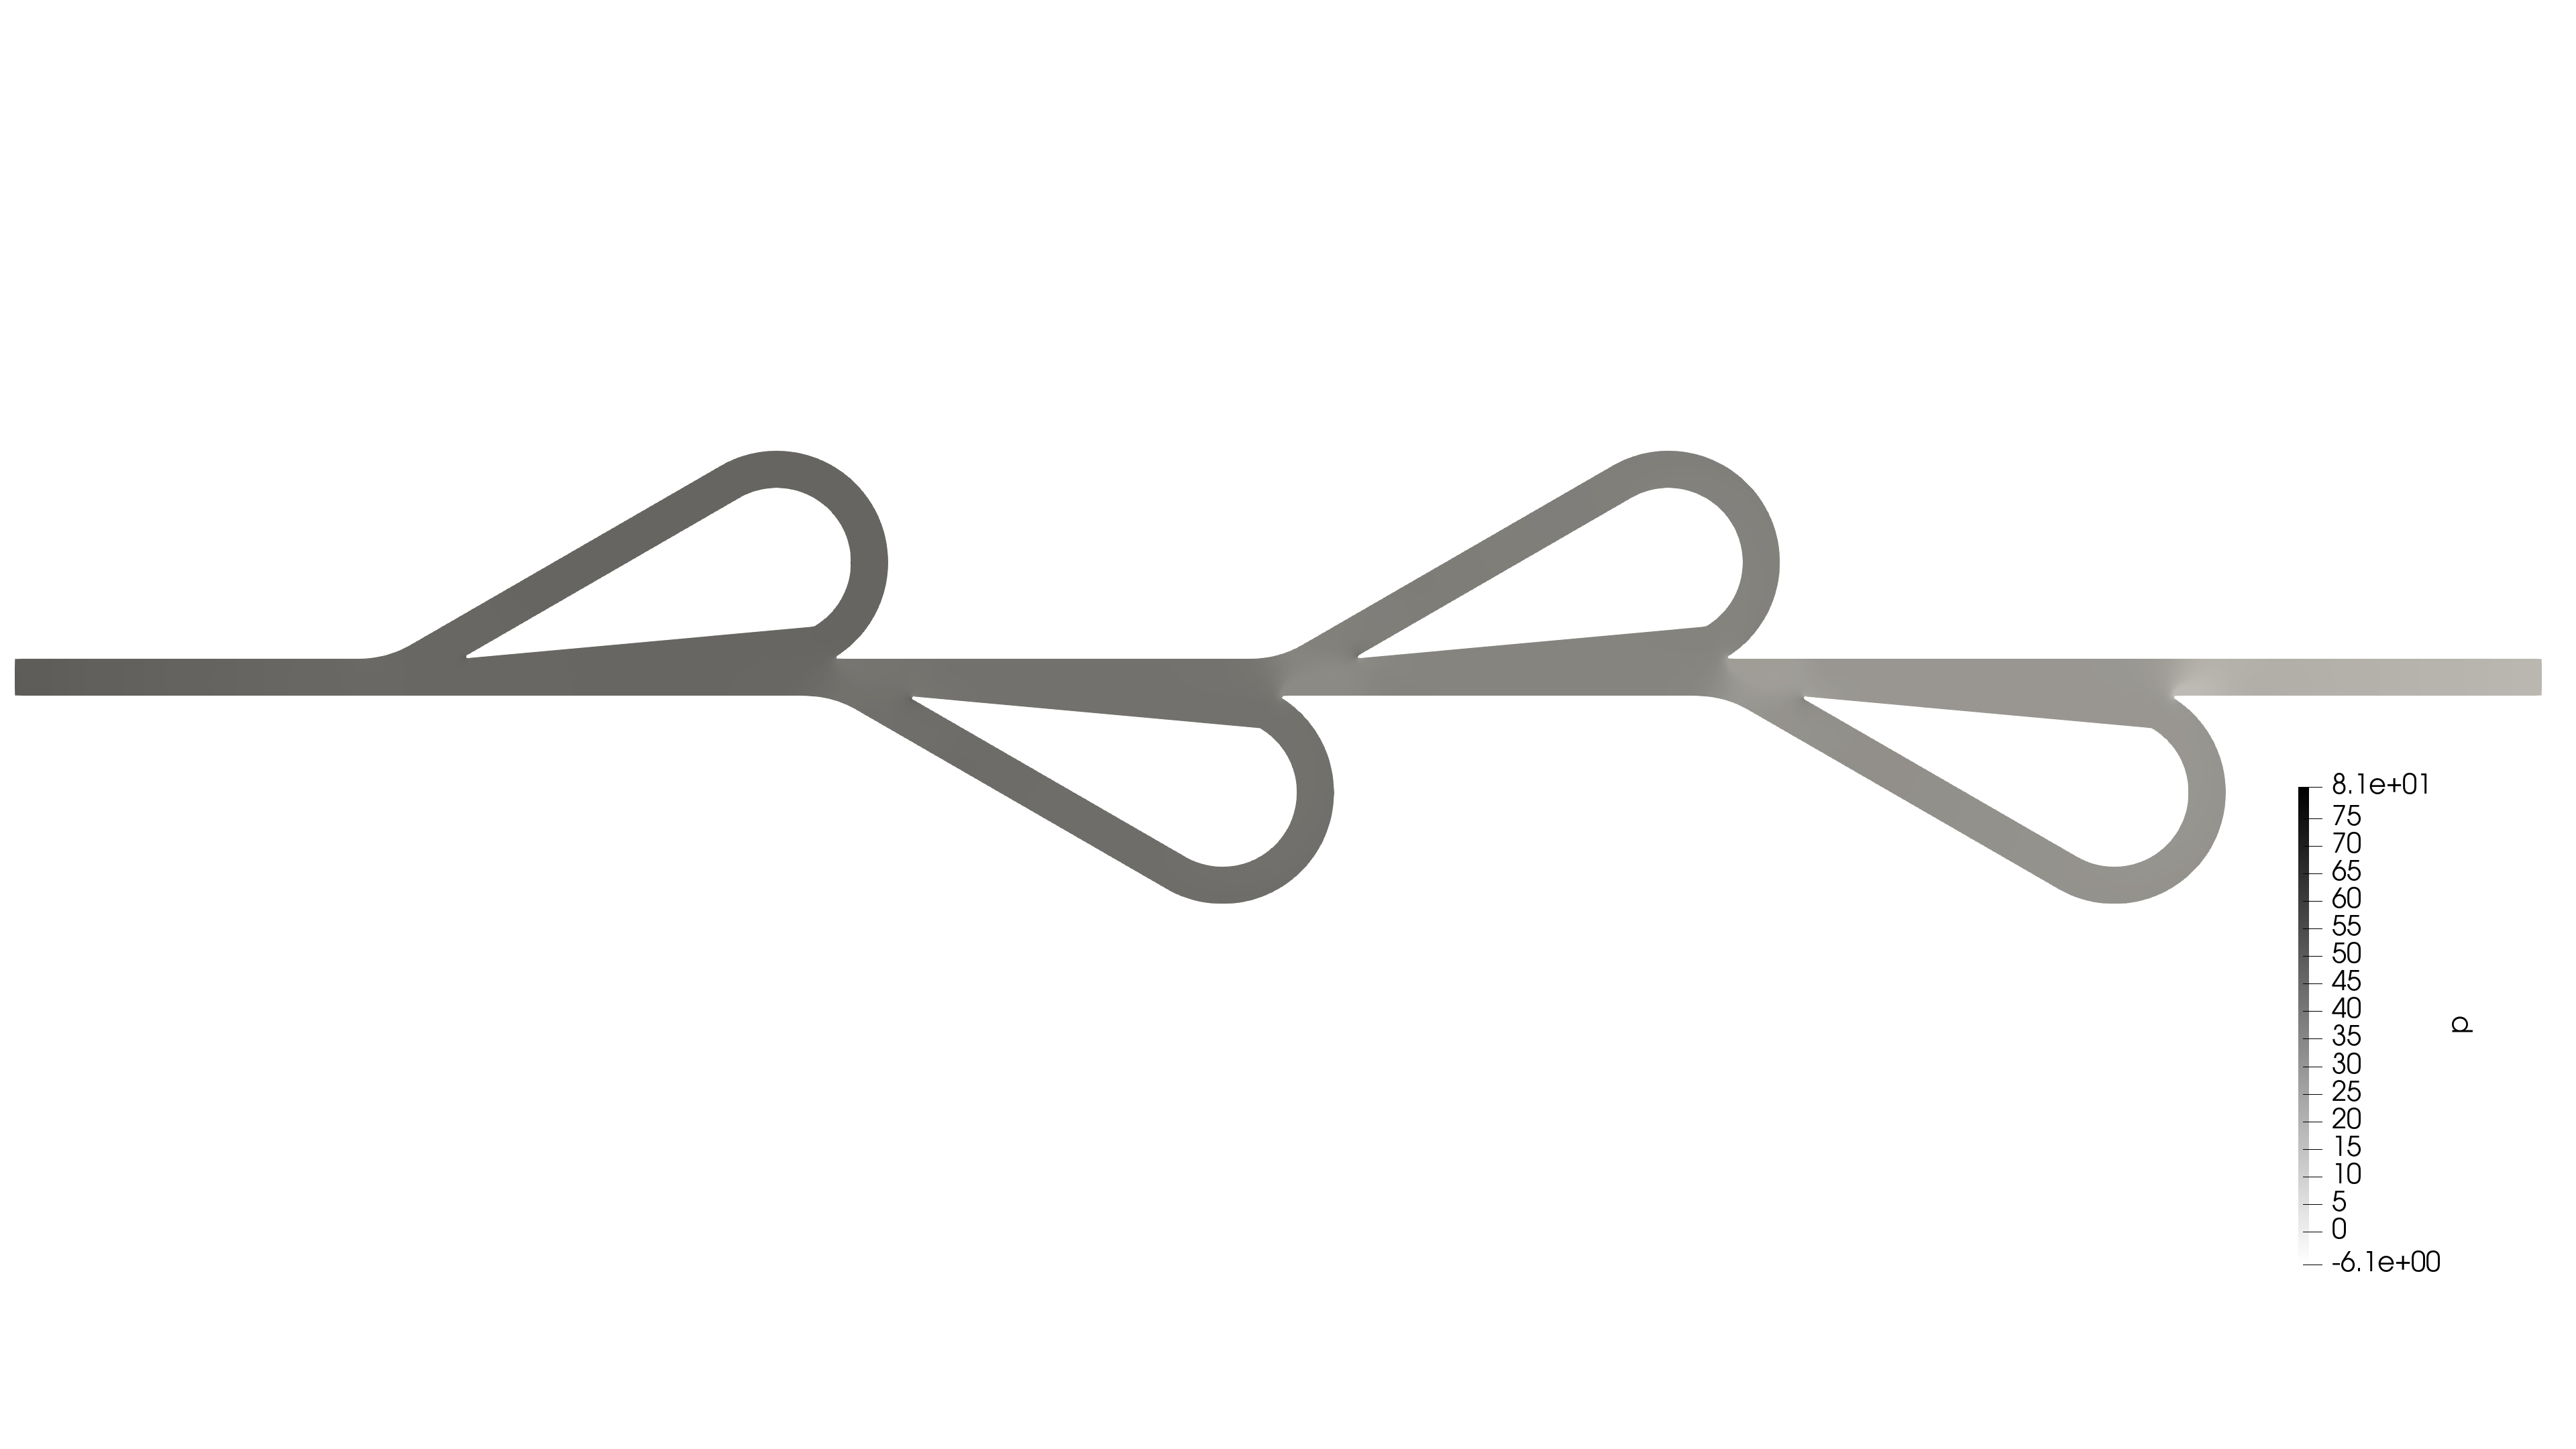
\includegraphics[width = 1\linewidth]{PFieldsReverse}
            \caption{Поле давление при обратном подключении.}
            \label{fig:PFieldsReverse}
        \end{figure}
        
        \begin{figure}[H]
            \centering
            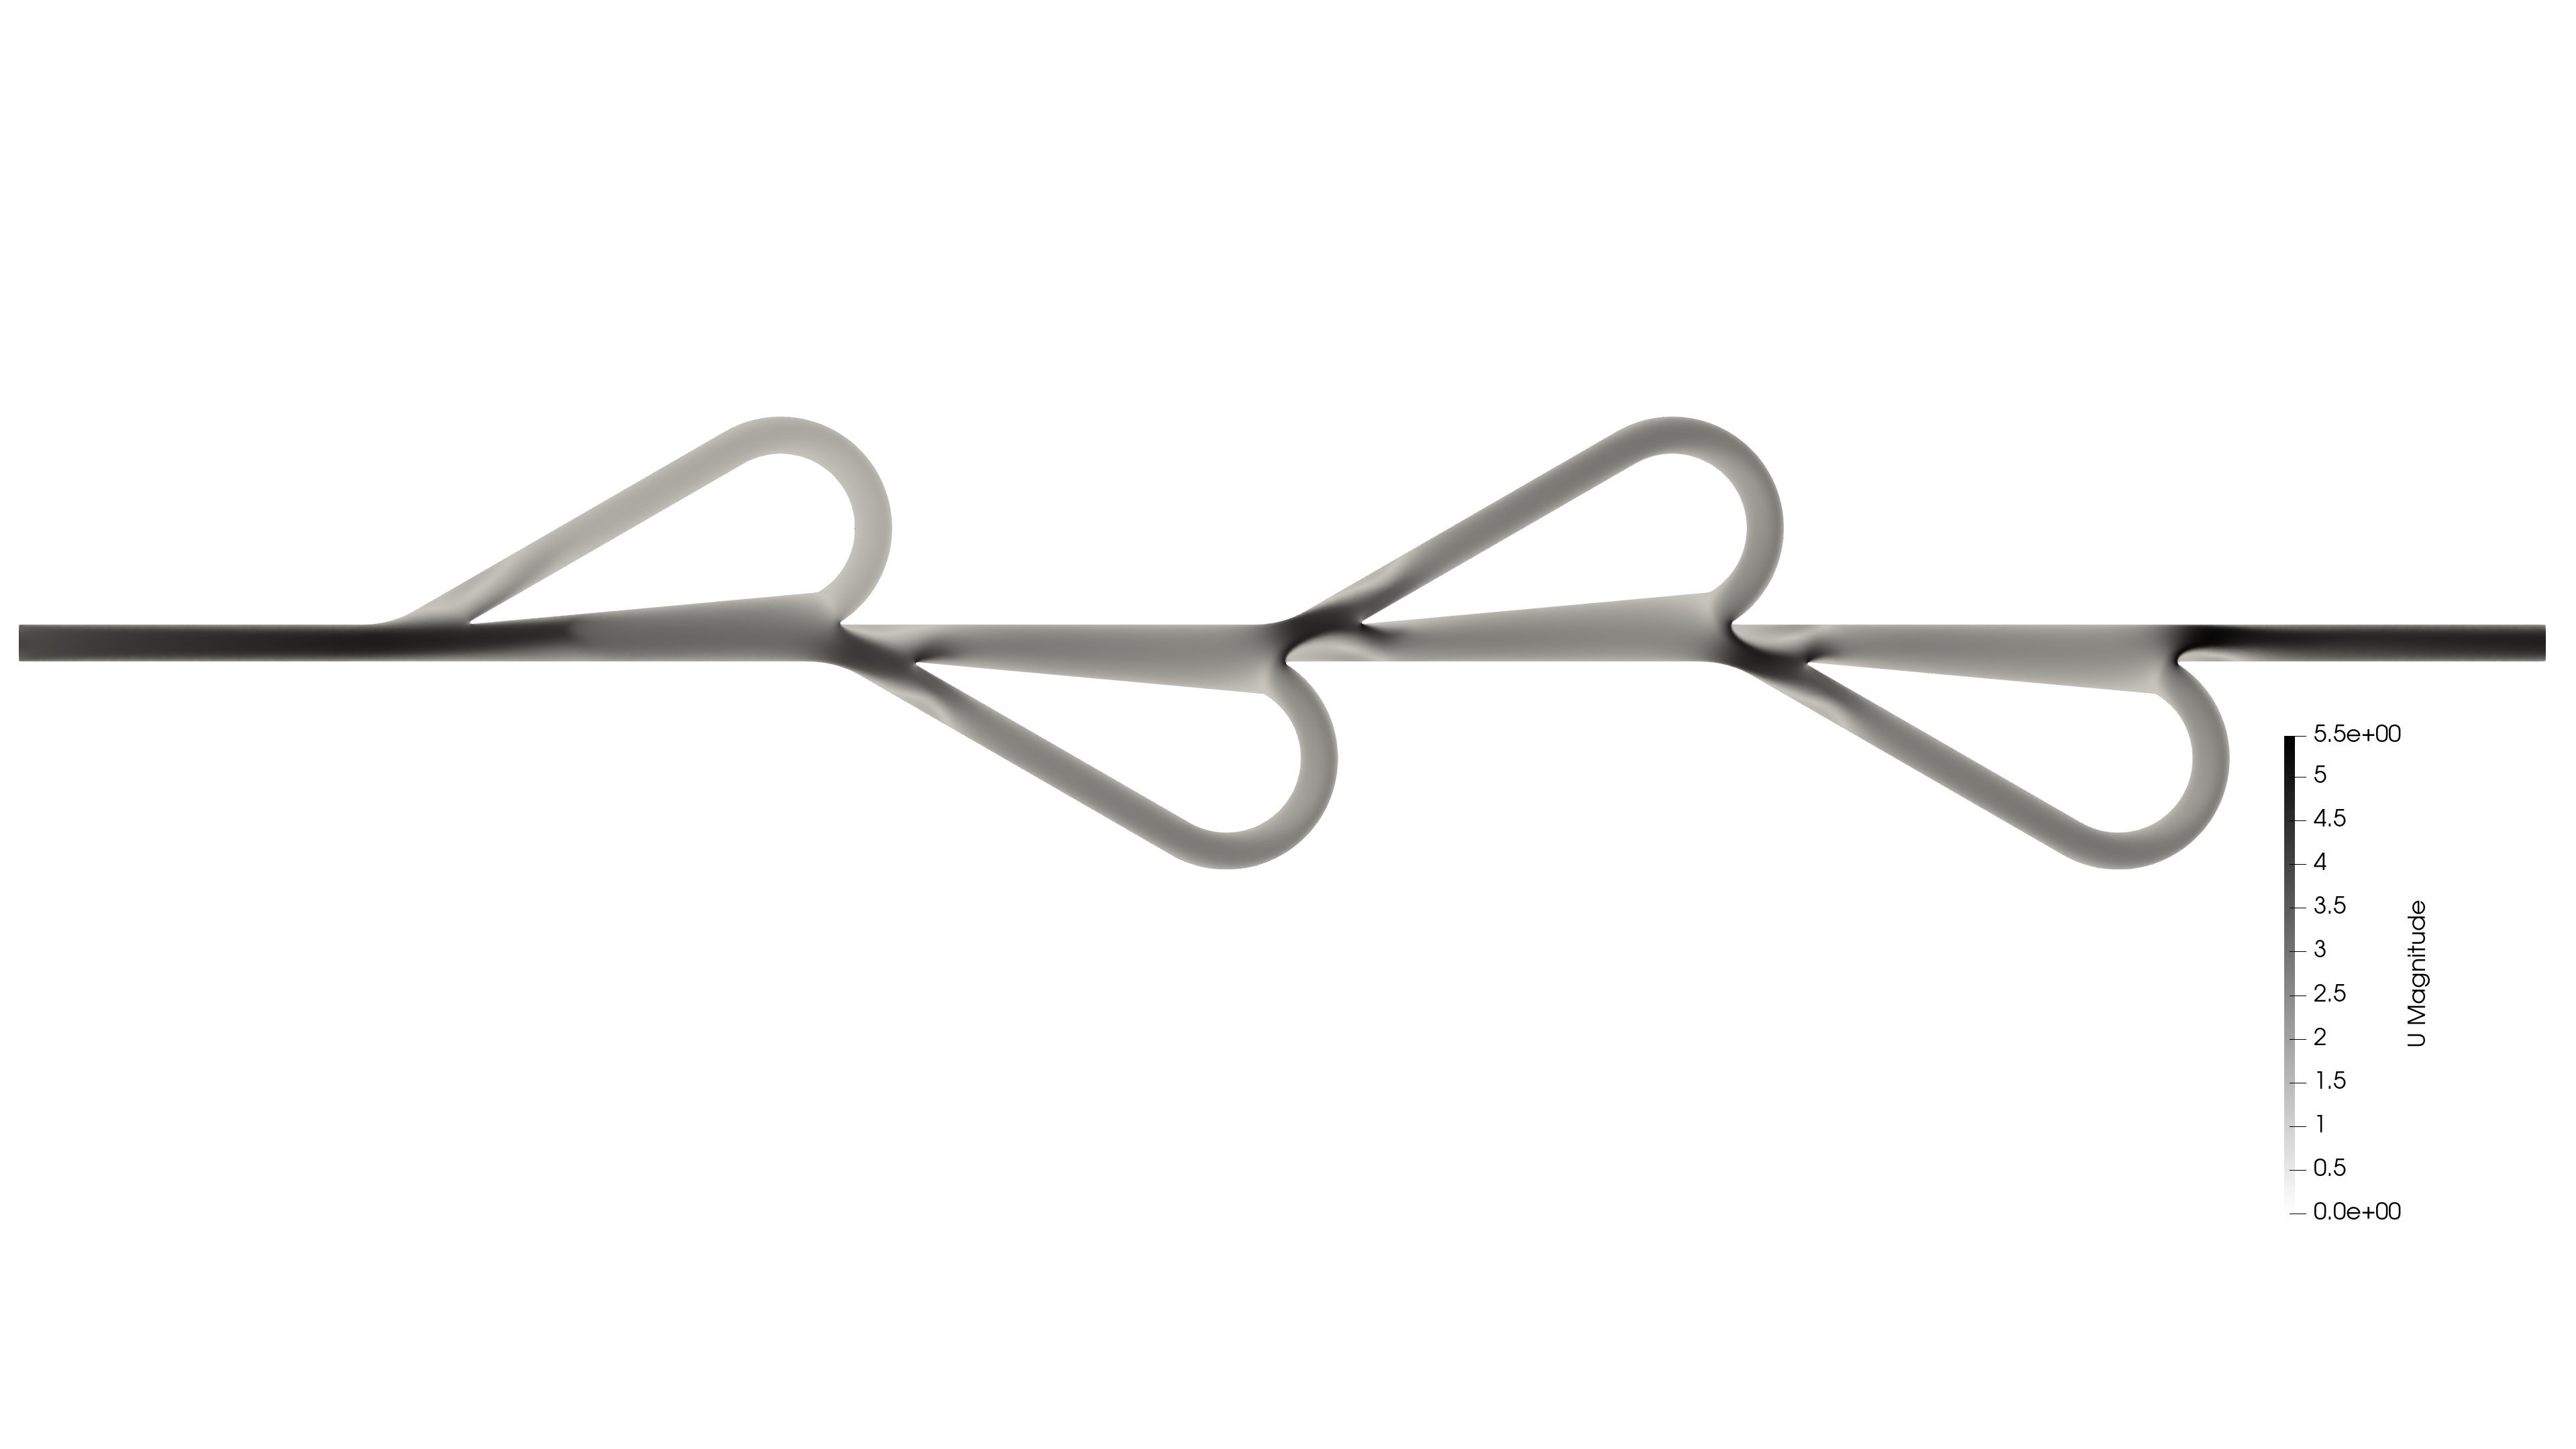
\includegraphics[width = 1\linewidth]{UFieldsReverse}
            \caption{После скорости при обратном подключении.}
            \label{fig:UFieldsReverse}
        \end{figure}
            
        Ход исследования сеточной сходимости. Было принято решение отталкиваться максимального размера ячейки. Каждая следующая сетка отличалась от предыдущей тем, что заданный максимальный размер ячейки отличался на 20 процентов. Таким образом мы получаем следующую таблицу: 
        \\
        \begin{table}[!htb]
            \begin{center}
                \caption{Результаты исследования сеточной сходимости.}
                \begin{tabular}{rccc}                 
                    \hline
                    №      & Максимальный размер ячейки, мкм & Кол-во элементов сетки  & $Di$ \\
                    \hline
                    \hline
                    1	& 100		& 728 607		& 1,213		\\
                    2	& 80		& 1 106 796	 	& 1,204		\\
                    3   & 64		& 2 072 292		& 1,197		\\
                    4	& 51,2		& 3 395 988		& 1,213		\\
                    5	& 40,96		& 5 116 005		& 1,222		\\
                    6	& 32,768	& 12 107 251	& 1,262		\\
                    \hline                   
                \end{tabular}
                \label{tab:tab1} 
            \end{center}
        \end{table}
        \\
        
        График зависимости диодности клапана Тесла от разрешения сетки, где мерой разрешения является количество элементов сетки, имеет вид:
        
        \begin{figure}[H]
            \centering
            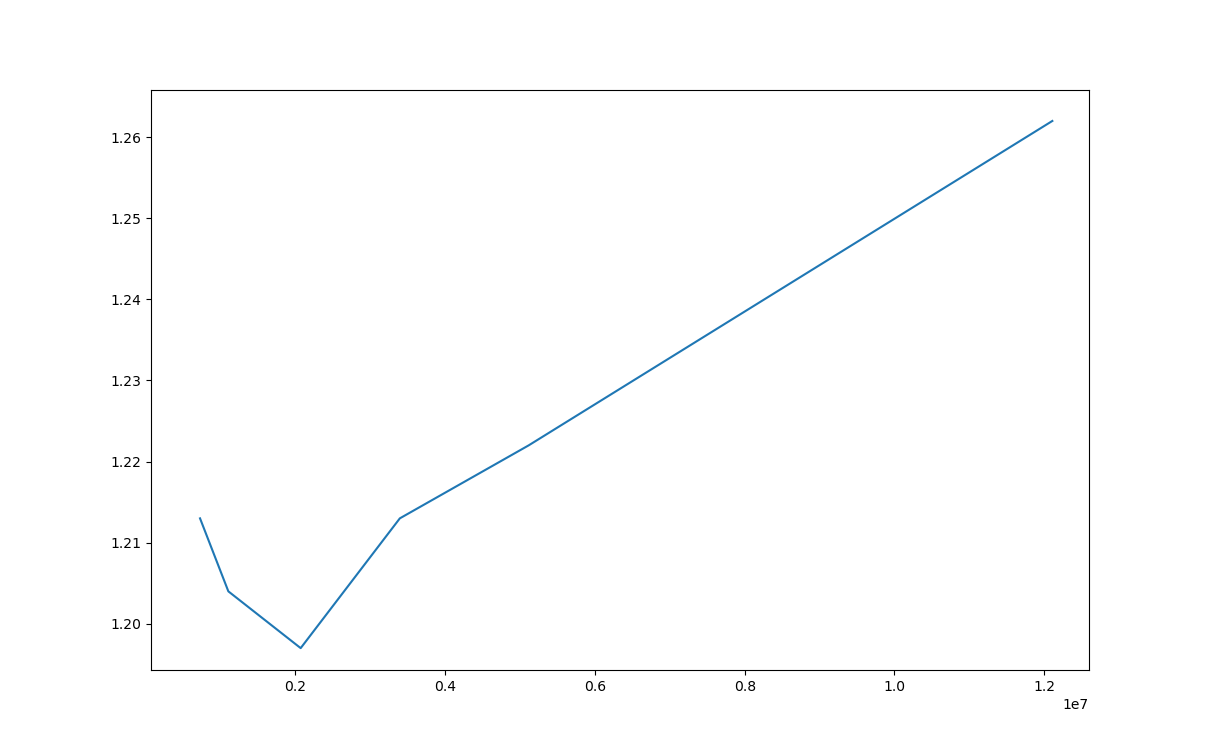
\includegraphics[width = 1\linewidth]{graphDi1}
            \caption{Зависимость диодности от разрешения сетки.}
            \label{fig:graphDi1}
        \end{figure}
                                    
        По графику (рис.~\ref{fig:graphDi1}) можно видеть, что с увеличением количества элементов сетки растет и диодность. Для того, чтобы сделать вывод о сеточной сходимости, нам надо добавить точек и выяснить, после какого разрешения диодность перестанет расти и начнет колебаться. Таблица с дополнительными точками будет иметь вид:
        \\
         \begin{table}[!htb]
            \begin{center}
                \caption{Результаты исследования сеточной сходимости с доп. точками.}
                 \begin{tabular}{rccc}
                     \hline
                     №      & Максимальный размер ячейки, мкм & Кол-во элементов сетки  & $Di$ \\
                     \hline
                     \hline
                     1	& 100		& 728 607		& 1,213		\\
                     2	& 80		& 1 106 796		& 1,204		\\
                     3  & 64		& 2 072 292		& 1,197		\\
                     4	& 51,2		& 3 395 988		& 1,213		\\
                     5	& 40,96		& 5 116 005		& 1,222		\\
                     6	& 40		& 5 602 384		& 1,287		\\
                     7	& 39,5		& 7 844 962		& 1,278		\\
                     8	& 39		& 9 039 949		& 1,288		\\
                     9	& 38		& 9 620 454		& 1,299		\\		
                     10	& 35		& 10 540 924	& 1,304		\\
                     11	& 32,768	& 12 107 251	& 1,262		\\
                     12	& 31,1296	& 12 896 528	& 1,311		\\
                     13	& 29,6		& 13 815 303	& 1,327		\\
                     14	& 28,6		& 14 401 893	& 1,310		\\
                     15	& 26		& 15 471 471	& 1,320		\\
                     16	& 25		& 16 085 501	& 1,330		\\
                     17	& 24	  	& 18 362 556	& 1,345		\\
                     18	& 23		& 22 476 068	& 1,327		\\
                     19	& 21		& 24 620 942	& 1,291		\\
                     20	& 19		& 28 765 237	& 1,3		\\
                     \hline
                     \label{fig:table2}
                 \end{tabular}
            \label{tab:tab2} 
            \end{center}
        \end{table}
         \\
         
         
         
%         \begin{figure}[H]
%             \centering
%             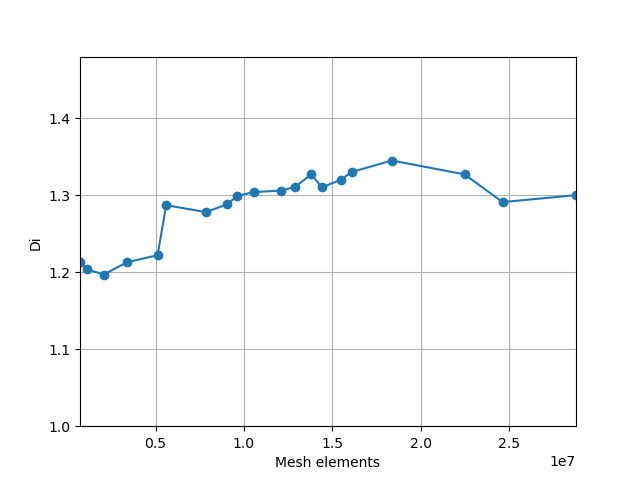
\includegraphics[width = 1\linewidth]{graphDi2}
%             \caption{Зависимость диодности от разрешения сетки c доп. точками.}
%             \label{fig:graphDi2}
%         \end{figure}           
         
         \begin{figure}[H]
             \centering
             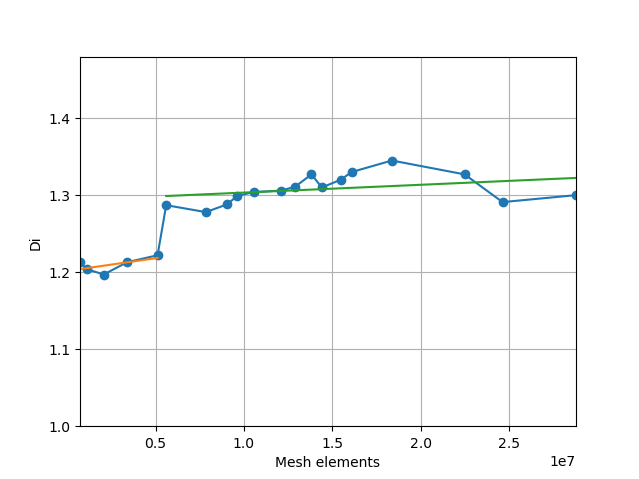
\includegraphics[width = 1\linewidth]{graphDiWithTrendLine}
             \caption{Линии тренда для зависимости диодности от количества элементов}
             \label{fig:graphDiWithTrendLine}
         \end{figure}     
         
         По представленным на графике (рис.~\ref{fig:graphDiWithTrendLine}) данным можно видеть, как с последующем увеличением разрешения сетки, диодность резко возрастает, однако, в последствии, рост диодности заметно замедляется. Исходя из этого, можно сделать вывод о сеточной сходимости. Достигая определенной плотности сетки, дальнейшее увеличение количества элементов не приведет к значительному улучшению решения, но потребует дополнительных вычислительных ресурсов. Добавленные линии тренда позволяют нам увидеть, что сетки до 5 млн элементов имеют рост диодности выше, чем сетки с более высокой плотностью, но среднее значение диодности у них меньше. Для дальнейшего параметрического исследования, нам следует выбрать сетку, плотность которой можно считать оптимальной. Для этого построим график зависимости диодности от максимального размера ячейки сетки.
         
                    
         
         \begin{figure}[H]
             \centering
             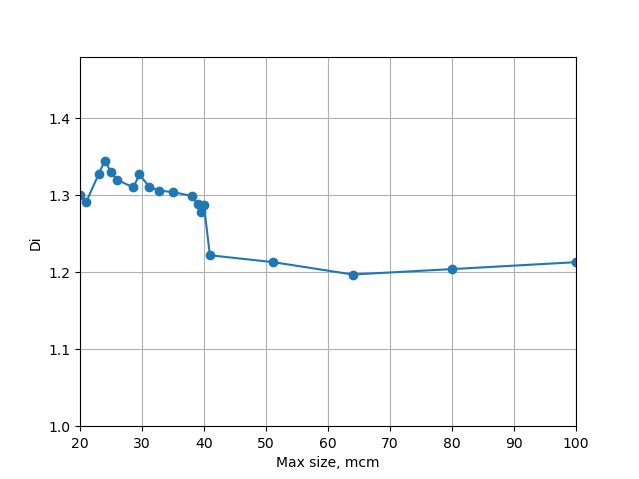
\includegraphics[width = 1\linewidth]{graphDiMaxSize}
             \caption{Зависимость диодности от максимального размера ячейки}
             \label{fig:graphDiMaxSize}
         \end{figure}
         
         Из графика (рис.~\ref{fig:graphDiMaxSize}) можно сделать вывод о том, что значительный прирост диодности происходит при максимальном характерном размере ячейки сетки равным 40 мкм. Этот размер мы и будем использовать при параметрическом исследовании. Что позволить нам получать более точные результаты оптимально задействовав вычислительные мощности. 

         \printbibliography

%        \section*{Список литературы.}
%        
%        1. Jin, Zhi-jiang; Gao, Zhi-xin; Chen, Min-rui; Qian, Jin-yuan . (2018). Parametric study on Tesla valve with reverse flow for hydrogen decompression. International Journal of Hydrogen Energy.
%        
%        2. Zhe Liu, Wen-Qi Shao, Yong Sun, Bo-Hua Sun (2022) Scaling law of
%        the one-direction flow characteristics of symmetric Tesla valve, Engineering Applications of
%        Computational Fluid Mechanics.
%        
%        3. E. Morganti, G.U.Pignatel, Microfluidics for the treatment of the hydrocephalus, 1st International Conference on Sensing Technology
%        November 21-23, 2005 Palmerston North, New Zealand.              
%        
%        4. Song, X., Cui, L., Cao, M., Cao, W., Park, Y.,Dempster, W. M. (2014). A CFD analysis of the dynamics of a direct-operated safety relief valve mounted on a pressure vessel. Energy Conversion and Management, 81, 407–419.
%        
%        5. Gamboa, A. R., Morris, C. J.,Forster, F. K. (2003). Optimization of the Fixed-Geometry Valve for Increased Micropump Performance. Fluids Engineering.
%        
%        6. Forster, F. K.,Williams, B. E. (2002). Parametric Design of Fixed-Geometry Microvalves: The Tesser Valve. Fluids Engineering.
%        
%        7. А. А. Гаврилов, А. А. Дектерев, А. В. Шебелев. Журнал вычислительной математики и математической физики, 2023, T. 63, № 4, стр. 533-547. ПРОСТОЙ КРИТЕРИЙ ОЦЕНКИ СЕТОЧНОЙ ДЕТАЛИЗАЦИИ ДЛЯ RANS МЕТОДОВ.      
                              
                      
            
    
    
\end{document}    